\section{Exploring Fourier Space}

The results for the phase and magnitude extraction are shown in figures \ref{fig:low-magnitude}, \ref{fig:high-magnitude}, \ref{fig:high-phase} and \ref{fig:low-phase}.

\begin{figure}[h!]
\centering
\begin{subfigure}{0.2\textwidth}
  \centering
  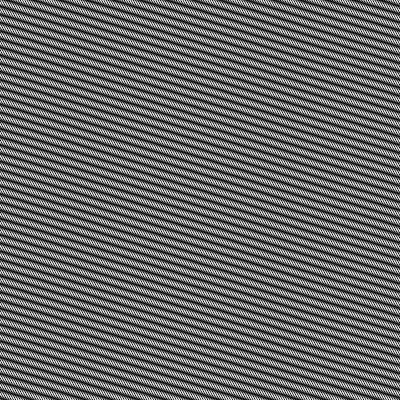
\includegraphics[width=0.95\linewidth]{output/magnitud_low_1.jpg}
  \caption{1st lowest}
\end{subfigure}%
\begin{subfigure}{0.2\textwidth}
  \centering
  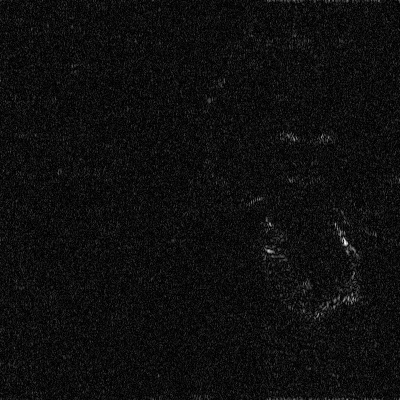
\includegraphics[width=0.95\linewidth]{output/magnitud_low_25.jpg}
  \caption{25 \% lowest}
\end{subfigure}%
\begin{subfigure}{0.2\textwidth}
  \centering
  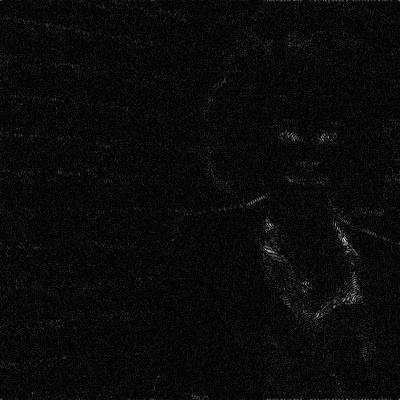
\includegraphics[width=0.95\linewidth]{output/magnitud_low_50.jpg}
  \caption{50 \% lowest}
\end{subfigure}%
\begin{subfigure}{0.2\textwidth}
  \centering
  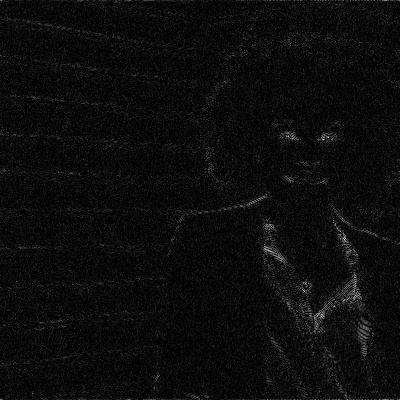
\includegraphics[width=0.95\linewidth]{output/magnitud_low_75.jpg}
  \caption{75 \% lowest}
\end{subfigure}%
\begin{subfigure}{0.2\textwidth}
  \centering
  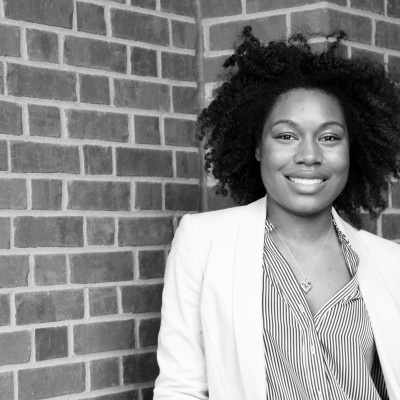
\includegraphics[width=0.95\linewidth]{output/magnitud_low_100.jpg}
  \caption{100 \% lowest}
\end{subfigure}%
 \caption{Low magnitude extraction}
\label{fig:low-magnitude}
\end{figure}

Getting the lowest values(figure~\ref{fig:low-magnitude})of the magnitude yields in images that shows groups of points that represents the woman of the original image. Note that the first image (the 1st lowest) seems to not have relation with the original image.

\begin{figure}[h!]
\centering
\begin{subfigure}{0.2\textwidth}
  \centering
  
\includegraphics[width=0.95\linewidth]{output/magnitud_high_1}
  \caption{1st highest}
\end{subfigure}%
\begin{subfigure}{0.2\textwidth}
  \centering
  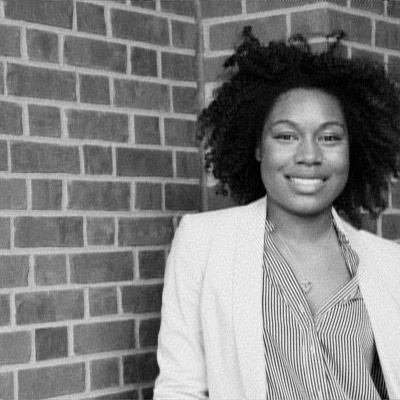
\includegraphics[width=0.95\linewidth]{output/magnitud_high_25}
  \caption{25 \% highest}
\end{subfigure}%
\begin{subfigure}{0.2\textwidth}
  \centering
  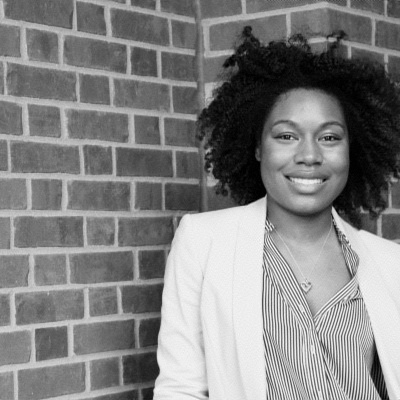
\includegraphics[width=0.95\linewidth]{output/magnitud_high_50}
  \caption{50 \% highest}
\end{subfigure}%
\begin{subfigure}{0.2\textwidth}
  \centering
  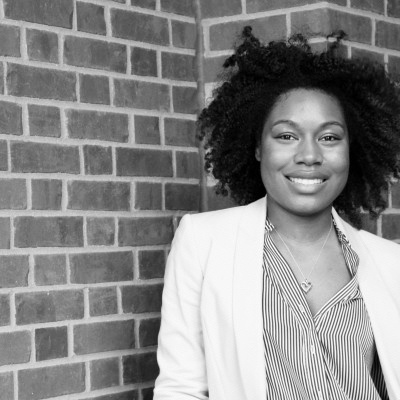
\includegraphics[width=0.95\linewidth]{output/magnitud_high_75}
  \caption{75 \% highest}
\end{subfigure}%
\begin{subfigure}{0.2\textwidth}
  \centering
  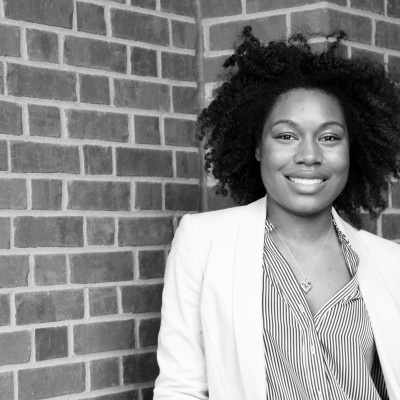
\includegraphics[width=0.95\linewidth]{output/magnitud_high_100}
  \caption{100 \% highest}
\end{subfigure}%
 \caption{High magnitude extraction}
\label{fig:high-magnitude}
\end{figure}

We can see in the figure \ref{fig:high-magnitude}, that the effect of taking the 1st greatest value creates an image that seems to not have relation with the original one, but, in the rest of images the difference is really small, it is just a little more clear while taking higher values.

\begin{figure}[h!]
\centering
\begin{subfigure}{0.2\textwidth}
  \centering
  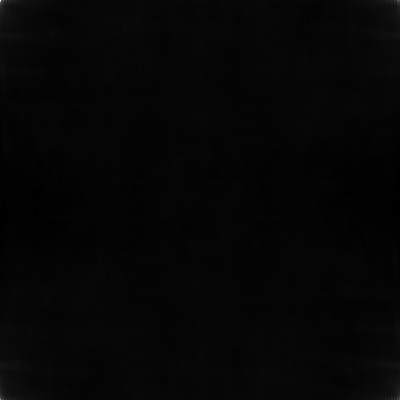
\includegraphics[width=0.95\linewidth]{output/phase_low_1.jpg}
  \caption{1st lowest}
\end{subfigure}%
\begin{subfigure}{0.2\textwidth}
  \centering
  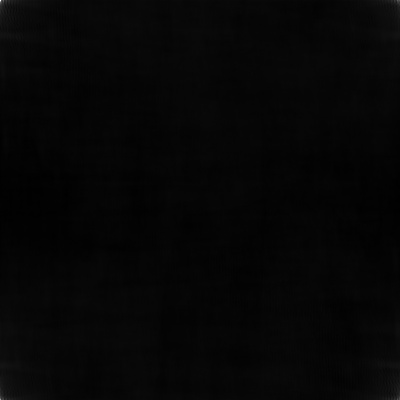
\includegraphics[width=0.95\linewidth]{output/phase_low_25.jpg}
  \caption{25 \% lowest}
\end{subfigure}%
\begin{subfigure}{0.2\textwidth}
  \centering
  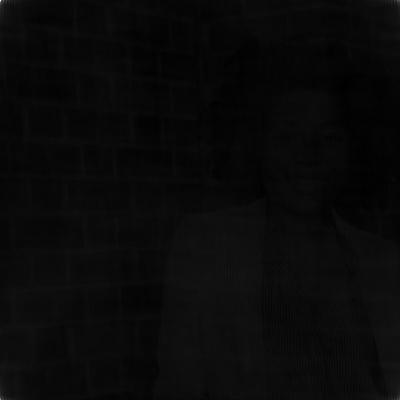
\includegraphics[width=0.95\linewidth]{output/phase_low_50.jpg}
  \caption{50 \% lowest}
\end{subfigure}%
\begin{subfigure}{0.2\textwidth}
  \centering
  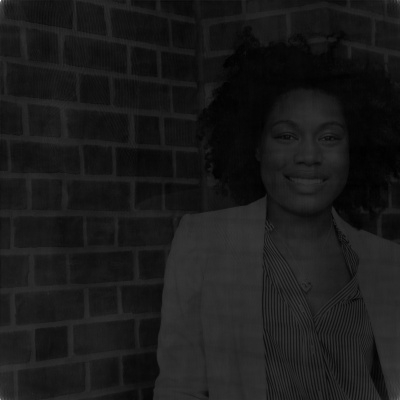
\includegraphics[width=0.95\linewidth]{output/phase_low_75.jpg}
  \caption{75 \% lowest}
\end{subfigure}%
\begin{subfigure}{0.2\textwidth}
  \centering
  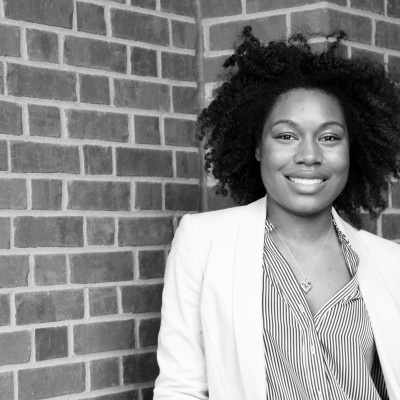
\includegraphics[width=0.95\linewidth]{output/phase_low_100.jpg}
  \caption{100 \% lowest}
\end{subfigure}%
 \caption{Low phase extraction}
\label{fig:low-phase}
\end{figure}

Also, we can see in the figure~\ref{fig:low-phase} that while we take less quantity of lower values, the intensity of the image is lower. This occurs because the phase carries a large part of the spatial information of the image, therefore, while we take more values, then major features of the image are preserved.

\begin{figure}[h!]
\centering
\begin{subfigure}{0.2\textwidth}
  \centering
  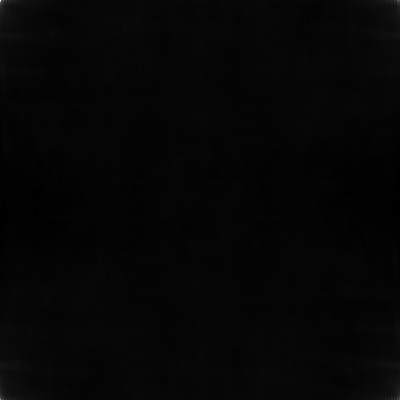
\includegraphics[width=0.95\linewidth]{output/phase_high_1.jpg}
  \caption{1st highest}
\end{subfigure}%
\begin{subfigure}{0.2\textwidth}
  \centering
  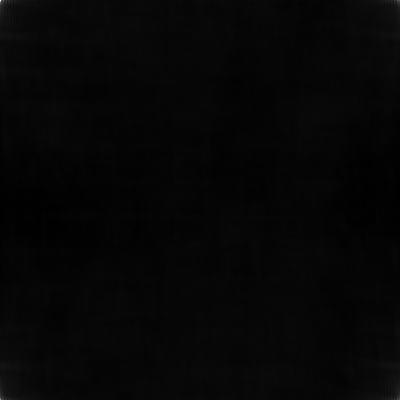
\includegraphics[width=0.95\linewidth]{output/phase_high_25.jpg}
  \caption{25 \% highest}
\end{subfigure}%
\begin{subfigure}{0.2\textwidth}
  \centering
  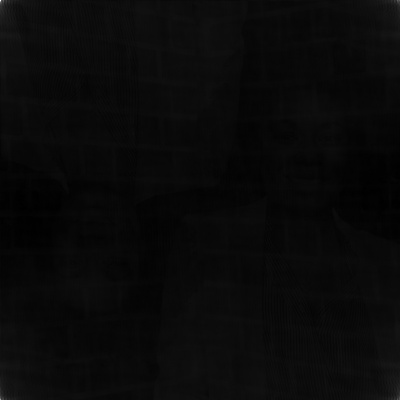
\includegraphics[width=0.95\linewidth]{output/phase_high_50.jpg}
  \caption{50 \% highest}
  \label{fig:high-phase-c}
\end{subfigure}%
\begin{subfigure}{0.2\textwidth}
  \centering
  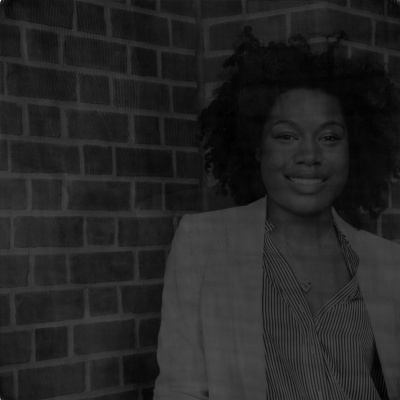
\includegraphics[width=0.95\linewidth]{output/phase_high_75.jpg}
  \caption{75 \% highest}
\end{subfigure}%
\begin{subfigure}{0.2\textwidth}
  \centering
  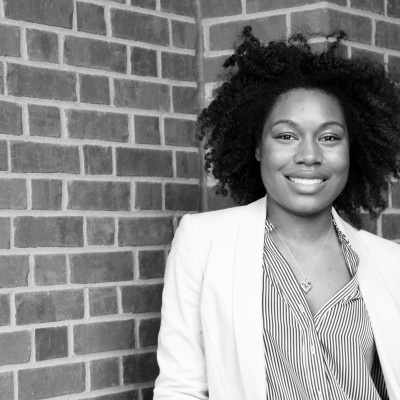
\includegraphics[width=0.95\linewidth]{output/phase_high_100.jpg}
  \caption{100 \% highest}
\end{subfigure}%
 \caption{High phase extraction}
\label{fig:high-phase}
\end{figure}
Similar to above, in the figure~\ref{fig:high-phase} we can see that the intensity of the image is less while taking less quantity of high values. Also we can see that in the sub figure~\ref{fig:high-phase-c} the image suffer a modification, creating a woman of inverted shape next to the original woman. This occurs because we take only high values altering the original spacial characteristics.

Comparing results from images \ref{fig:low-magnitude} and \ref{fig:low-phase}, we can see that the changes in phase have a bigger effect (e.g. we lose a lot of information), moreover, comparing \ref{fig:high-magnitude} and \ref{fig:high-phase}, the results of getting the highest values in the magnitude seems to not have any effect, on the other hand, getting the 75 \% of the highest phase values yields in big changes. Thus the phase is more important than the magnitude.

